%%%%%%%%%%%%%%%%%%%%%%%%%%%%%%%%%%%%%%%%%%%%%%%%%%%%%%%%%%%%%%%%%%%%%%%%%%
%%%%%%%%%%               (Tanjona Radonirina)                 %%%%%%%%%%%%
%%%%%%%%%%%%%%%%%%%%%%%%%%%%%%%%%%%%%%%%%%%%%%%%%%%%%%%%%%%%%%%%%%%%%%%%%%
\documentclass[twocolumn,secnumarabic,amssymb, nobibnotes, aps, prd,10pt]{revtex4-1}

\newcommand{\revtex}{REV\TeX\ }
\newcommand{\classoption}[1]{\texttt{#1}}
\newcommand{\macro}[1]{\texttt{\textbackslash#1}}
\newcommand{\m}[1]{\macro{#1}}
\newcommand{\env}[1]{\texttt{#1}}
\setlength{\textheight}{9.5in}

\usepackage{slashed}
\newcommand{\ignore}[1]{}

\usepackage{amsmath,multirow}
\setcounter{secnumdepth}{3}

\usepackage{color}
\definecolor{azure}{rgb}{0.0, 0.44, 1.0}
\definecolor{ceruleanblue}{rgb}{0.16, 0.32, 0.75}

\usepackage{hyperref}
\hypersetup{
	colorlinks=true,
	linkcolor=red,
	citecolor=azure,
	urlcolor=cyan,
}

\usepackage{mhchem}
\usepackage{graphicx}
\usepackage{wrapfig}
\usepackage{sidecap}
\usepackage{subcaption}	 
\usepackage{lipsum}  

% Define path to plots
\graphicspath{{../pythonCode/analysis/plots/Osc3Neutrinos/}}

\newcommand{\kt}[1]{\vert #1 \rangle}
\newcommand{\bt}[2]{\langle #1 \vert #2 \rangle}
\newcommand{\bkt}[3]{\langle #1 \vert #2 \vert #3 \rangle}

\newcommand{\Eq}[1]{Eq.$\:$(\ref{#1})}
\newcommand{\myref}[1]{Ref.$\:$\cite{#1}}
\newcommand{\Fig}[1]{Fig.$\:$\ref{#1}}
\newcommand{\App}[1]{App.$\:$\ref{#1}}
\newcommand{\SubApp}[2]{App.$\:$\ref{#1}.\ref{#2}}
\newcommand{\Sec}[1]{Section$\:$\ref{#1}}

% For units
\usepackage{siunitx}
\newcommand{\gev}[1]{\SI{#1}{\giga\electronvolt}}
\newcommand{\tev}[1]{\SI{#1}{\tera\electronvolt}}
%************************************************************************************************************

\begin{document}

\title{\texorpdfstring{Phenomenological Introduction to Neutrino Oscillations}{Phenomenological Introduction to Neutrino Oscillations}}

\author{Tanjona R.\ Rabemananjara}
\email{tanjona.rabemananjara@mi.infn.it}
\affiliation{Universita degli Studi di Milano \\
Via Celoria 16, Milano 20133, Italy}

\maketitle
%\tableofcontents

%%%%%%%%%%%%%%%%%%%%%%%%%%%%%%%%%%%%%%%%%%%%%%%%%%%%%%%%%%%%%%%%%%%%%%%%%%%%%%%%%%%
\section{Introduction}

Since the idea of neutrino oscillations has been hypothesized by Potencorvo in 1957
\cite{Potencorvo:1957cp, Xontecorvo:1957qd}, important experimental and theoretical
developments have emerged from the study of the properties of neutrino. Chief among
these findings is the fact that there has to be physics beyond the Standard Model 
(SM). The theoretical framework of neutrino mixing and masses for explaining neutrino
oscillations his now firmly established. To date, the size of the mass-squared 
difference together with the mixing angles have been measured. However, despite the
incredible precision (better than $10 \%$) in measuring the mass-mixing parameters, 
the picture is not complete yet. The ordering and scale of the neutrino masses is not
fully understood yet along with the value of the Dirac-phase $\delta$. Furthermore, 
flavor oscillations do not probe the nature of the neutrino fields-whether it is Dirac 
or Majorama.

Various programs worldwide are currently being pursued in order to provide more
experimental capabilities to tackle these issues \cite{Acciarri:2015uup, Antonello:2015lea, 
An:2015jdp, Djurcic:2015vqa, Adamson:2016tbq, Kim:2014rfa, Adamson:2016xxw, Abe:2015awa,
Adams:2013qkq}. For instance, in order to make a precise measurement of the Dirac phase, an 
unprecedented amount of neutrino oscillation data will be needed in order to reduce the 
statistical errors. This could only be achieved with new detectors with larger mass and 
higher power beams.

This summary project consists of four sections. In \Sec{sec:experiment}, we give a short
overview of the experimental probes that led to the discovery of the neutrino oscillations.
In \Sec{sec:theory}, we give the theoretical aspects of the neutrino oscillation probabilities
by highlighting the definition of survival probability. Phenomenological results are presented
in \Sec{sec:pheno}. Finally, conclusions and discussion on the remaining opened problems are
drawn in \Sec{sec:conclusion}.


\section{Experimental probe of neutrino oscillation phenomenon}
\label{sec:experiment}

Experimental evidence of neutrino oscillations can be studied from various sources:
atmospheric neutrinos, nuclear-reactor neutrinos, and neutrino-antineutrino accelerator
beams. The atmospheric neutrinos result from the interaction of cosmic rays and the
atmosphere and mostly come from the following reactions:
\begin{align}
\pi^\pm  &\longrightarrow \mu^\pm + \nu_\mu / \bar{\nu}_\mu, \\
\mu^\pm  &\longrightarrow e^\pm + \nu_e / \bar{\nu}_e + \bar{\nu}_\mu / \nu_\mu .
\end{align}
Production of electron-flavor antineutrino $\bar{\nu}_e$ can be accessed from nuclear
reactor experiments in which the $\bar{\nu}_e$ are released from the fission of the 
main isotopes $\left( \ce{^{235}U}, \ce{^{239}Pu} \right)$ used in the nuclear reactors.
Finally, (anti-)neutrinos can be produced from various collider experiments such as
CERN, FNAL, and the Los Alamos Neutron Science Center.

Historically, one of the earliest indication of neutrino oscillations was found in 
atmospheric neutrino experiments that used radeiochemical techniques with the Homestake
detector \cite{Cleveland:1998nv}. These experiments measure a flux of electron-flavor 
neutrinos $\nu_e$, originating from the sun, that was significantly lower than the 
one expected by the Standard Solar Model (SSM). Because solar $\nu_e$ oscillate to 
different flavors, the detectors which are only sensitive to $\nu_e$ detect smaller 
number of events. This phenomenon has been known as the \emph{solar neutrino problem} 
and has been confirmed by different neutrino experiments such as GALLEX 
\cite{Hampel:1996qd, Anselmann:1993mh}, Kamiokande \cite{Hirata:1988ad, Hirata:1991ub, 
Fukuda:1996sz}, and Super-Kamiokande \cite{Fukuda:1998fd, Giunti:1999qm}.

The first evidence of neutrino oscillations has been established by studying the 
atmospheric neutrinos with water \cite{Fukuda:1998mi, Ashie:2004mr} (Kamiokande and 
Sper-Kamiokande) in 1998. The data exhibit a zenith angle $\theta$ dependent deficit of 
$\nu_\mu$ which is inconsistent with calculations of neutrino atmospheric fluxes and 
cannot be explained by the experimental biases and uncertainties. Indeed, if neutrinos
do not oscillate, the number of observed atmospheric neutrino is predicted to be
uniform.
\begin{figure}
\centering
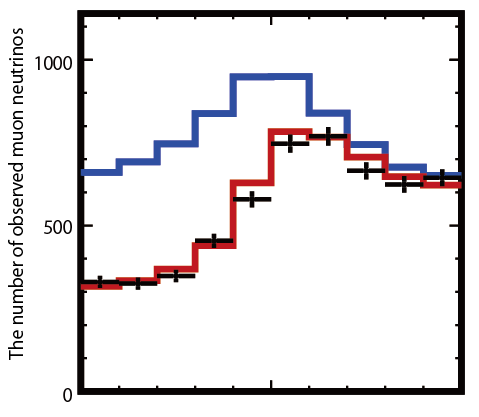
\includegraphics[scale=0.425]{zenith}
\caption{Observed muon-flavor neutrino from the Super-Kamiokande experiment. The \emph{blue}
curve represents the expected number of event without neutrino oscillation, the \emph{red}
curve represents the number of events in case of neutrino oscillation, and the \emph{black}
crosses represent the observed number of events in the Super-Kamiokande detector.}
\label{fig:superKami}
\end{figure}
In \Fig{fig:superKami} we see the number of observed muon-flavor neutrinos as a function of
the zenith angle $\cos (\theta)$ from the Super-Kamiokande analyses. This results show that
the number of \emph{upward} going muon neutrinos generated from the outer-atmosphere is half 
of the number of \emph{downward} going muon neutrino.

This observation suggested that neutrinos change flavors as they propagate from their source,
(through the medium), to the detectors. Such a mechanism of flavor changes require that the
neutrinos have more than one mass state which is not allowed by the SM. For this reason, the
neutrino oscillation provided a direct measurement of physics beyond the SM. Hence, the search
for understanding of the properties of the neutrinos is considered as one of the most important
directions for the search for new physics. To date, more than 40 different experiments is
dedicated to the investigation of the problem of neutrino masses and mixing.


\section{Theoretical framework}
\label{sec:theory}

Neutrinos interacts with other particles via weak interactions which are described
by the charge current (CC) and neutral current (NC) interaction Lagrangians 
\cite{Bilenky:1998dt}:
\begin{align}
\mathcal{L}_{CC} &= - \frac{g}{2 \sqrt{2}} \mathcal{J}^{CC}_\rho W^\rho + h.c, \\
\mathcal{L}_{NC} &= - \frac{g}{2 \cos(\theta_W)} \mathcal{J}^{NC}_\rho Z^\rho,
\end{align}
where $g$ represents the $SU(2)_L$ gauge coupling constant and $\theta_W$ the weak
angle. Furthermore, the charged and neutral current that are respectively denoted
by $\mathcal{J}^{CC}_\rho$ and $\mathcal{J}^{NC}_\rho$ are defined as:
\begin{align}
\mathcal{J}^{CC}_\rho &= 2 \sum_{l} \bar{\nu}_{lL} \gamma_\rho l_L + \cdots, \\
\mathcal{J}^{NC}_\rho &= \sum_{l} \bar{\nu}_{lL} \gamma_\rho \nu_{lL} + \cdots,
\end{align}
where the charged leptonic field $l$ can be one of the neutrino flavors $(e, \mu, \tau)$
with mass $m_l$. Notice that we have only written explicitly terms containing the neutrino
fields.

If neutrinos have zero-masses, the left-handed neutrino field $\nu_{\alpha L}$
with flavor $\alpha$ can be written as a superposition of the left-handed components
$\nu_{iL}$ of the neutrino field with mass $m_i$. In an ultra-relativistic scenario, we
have:
\begin{align}
\nu_{\alpha L} = U_{\alpha i} \nu_{i L}
\label{eq:superposition}
\end{align} 
where repeated indices are summed over. Henceforth, we use Greek letters to refer to
the neutrino masses and Latin letters to refer to the flavours. The neutrino masses
$i$ runs from $1$ to $N$ where $N$ denotes the number of massive neutrinos. In this
project, we are only going to focus in the case $N=3$.

In \Eq{eq:superposition}, $U$ is a unitary matrix. This implies that the flavor eigenstate
$\kt{\nu_\alpha}$ can be written as a superposition of different mass eigenstates $\kt{\nu_i}$
in the following way:
\begin{align}
\kt{\nu_{\alpha L}} &= U^\star_{\alpha i} \kt{\nu_i}, \\
\kt{\bar{\nu}_{\alpha L}} &= U_{\alpha i} \kt{\bar{\nu}_i}.
\end{align}
Assuming that we have three $(03)$ massive neutrinos, the mixing unitary matrix $U$ can 
be written as:
\begin{align}
U = & \left(\begin{array}{ccc}
1 & 0 & 0 \\
0 & c_{23} & s_{23} \\
0 & -s_{23} & c_{23}
\end{array}\right)\left(\begin{array}{ccc}
c_{13} & 0 & s_{13} e^{\mathrm{i} \delta_{13}} \\
0 & 1 & 0 \\
-s_{13} e^{\mathrm{i} \delta_{13}} & 0 & c_{13}
\end{array}\right) , \nonumber \\
& \left(\begin{array}{ccc}
c_{12} & s_{12} & 0 \\
-s_{12} & c_{12} & 0 \\
0 & 0 & 1
\end{array}\right)\left(\begin{array}{ccc}
1 & 0 & 0 \\
0 & e^{ \mathrm{i} \delta_{13} } & 0 \\
0 & 0 & 1
\end{array}\right)
\label{eq:evolution_matrix}
\end{align}
where $c_{ij} = \cos(\theta_{ij})$ and $s_{ij} = \sin(\theta_{ij})$. Here, $\theta_{ij}$
denote the mixing angles while $\delta$ denotes the Dirac-type CP-phase (often denoted 
here as $\delta_{CP}$. Defining $\Delta_{ij} = m_i^2 - m_j^2$ and ordering the masses 
such that $\Delta_{21}^2 > 0$ and $\Delta_{21}^2 < \Delta_{31}^2$, we have the following 
constraints:
\begin{align}
0 \leq \theta_{ij} \leq \frac{\pi}{2} \quad (i \neq j), \quad 0 \leq \delta \leq 2 \pi .
\end{align}


\subsection{Neutrino evolution equation in vacuum and in matter}
\label{subsec:evoleq}

The evolution equation of a generic neutrino state $\kt{\nu(t)}$ is described by a
Shrödinger-like equation:
\begin{align}
\mathrm{i} \partial_t \kt{\nu_\alpha(t)} = H \kt{\nu_\alpha(t)},
\end{align}
where $H$ represents the Hamiltonian operator. Expressed in the flavor eigenstate
basis $\kt{\nu_\alpha}$, the above equation translates into
\begin{align}
\mathrm{i} \partial_t \nu^{(f)}(t) = H^{(f)} \nu^{(f)}(t),
\end{align}
where $v^{(f)}(t)$ denotes the vector describing the flavor content of the neutrino state
$\kt{\nu(t)}$. Elements of the Hamiltonian matrix $H^{(f)}$ are given by
\begin{align}
H^{(f)}_{\alpha \beta} = \bkt{\nu_\alpha}{H}{\nu_\beta}.
\end{align}
In the mass eigenstate basis, the vacuum Hamiltonian $H^{(m)}$ (where $m$ indicates the
mass eigenstate representation) is determined in terms of the neutrino masses
\begin{align}
H^{(m)}_{vac} &= \mathrm{diag} \left( \sqrt{\vec{p}^2 + m_1^2}, \sqrt{\vec{p}^2 + m_2^2},
\sqrt{\vec{p}^2 + m_3^2} \right), \nonumber \\
&\approx \vert \vec{p} \vert + \frac{1}{2 \vert \vec{p} \vert} \mathrm{diag} \left( m_1^2, 
m_2^2, m_3^2 \right).
\end{align}
In the first equality we assumed that the neutrino state $\kt{\nu (t)}$ can be described
as a superposition of states with fixed momentum $\vec{p}$. In the last line, we used the
ultra-relativistic approximation $\sqrt{\vec{p}^2 + m_i^2} \sim \vert \vec{p} \vert + m_i^2
/2 \vert \vec{p} \vert$. The new Hamiltonian in the flavor eigenstates therefore reads
\begin{align}
H^{(f)}_{\alpha \beta, vac} = U_{\alpha i} H^{(m)}_{ij, vac} U^\dagger_{i \beta}
\end{align}

In the presence of matter, we have to add the vacuum Hamiltonian an effective potential
$V$ in the evolution equation
\begin{align}
i \partial_t \kt{\nu (t)} = \left( H_{vac} + V \right) \kt{\nu (t)},
\end{align}
where in the context of SM, the effective potential is a matrix that is diagonal in the
flavor basis $V^{(f)} = \mathrm{diag} \left( V_e, V_\nu, V_\tau \right)$.


\subsection{Survival probability}
\label{subsec:survival}

Assuming that a neutrino is created a a time $t_0 = 0$ at a point $x_0 = 0$, the flavor
state $\kt{\nu (t)}$ in the flavor eigenstate basis can be written as 
\begin{align}
\nu^{(f)} (0) = \left( \bt{\nu_e}{\nu(0)}, \bt{\nu_\mu}{\nu(0)}, \bt{\nu_\tau}{\nu(0)}
\right)^\mathrm{T}.
\end{align}
After some interval of time $t$ at a given point $x$, its flavor has evolved  according to
\begin{align}
\nu^{(f)} (x) = S^{(f)} (x) \nu^{(f)}(0),
\end{align}
where the evolution operator $S$ is expressed as
\begin{align}
S^{(f)} = T \left[ \mathrm{exp} \left( - \mathrm{i} \int_{0}^{x} \mathrm{d}\tilde{x} \:
H^{(f)} (\tilde{x}) \right) \right].
\end{align}
Recall that in the ultra-relativistic limit $x \approx t$. In the above equation, 
$\mathrm{T}$ represents the time ordering operator. Therefore, the probability to detect 
a neutrino of flavor $\nu_\beta$ at a distance $L$ from its initial position (where its 
initial flavor is known) is given by
\begin{align}
P (\nu_\beta \longleftarrow \nu_\alpha) = \vert S^{(f)}_{\beta \alpha} \vert^2.
\label{eq:prob_s}
\end{align}
This implies that the survival probability $P (\nu_\alpha \longleftarrow \nu_\alpha)$
is given by the following
\begin{align}
P (\nu_\alpha \longleftarrow \nu_\alpha) = 1 - P (\nu_\beta \longleftarrow \nu_\alpha).
\end{align}
The above expression is a consequence of the unitarity of the mixing matrix 
$\sum_\beta P (\nu_\beta \longleftarrow \nu_\alpha) = 1$.


\subsection{Vacuum neutrino oscillations}
\label{subsec:2neutrinoOsc}

As it was presented in the previous section, in vacuum the neutrino Hamiltonian $H$ is
constant. Hence, the evolution operator can be written as
\begin{align}
S^{(f)} = U S^{(m)} U^\dagger .
\end{align}
The evolution operator in the mass eigenstate (denoted by the upper-script $m$) is a 
diagonal matrix that is function of $\phi_i = -m_i^2 x / 2 \vert \vec{p} \vert$,
\begin{align}
S^{(m)} = \mathrm{diag} \left( \mathrm{exp}(i \phi_1), \mathrm{exp}(i \phi_2), 
\mathrm{exp}(i \phi_3) \right) .
\end{align}
Using \Eq{eq:prob_s}, the probability of observing a neutrino of flavor 
$\nu_\alpha$ to change into a neutrino of flavor $\nu_\beta$ is given by the following:
\begin{align}
P (\nu_\beta \longleftarrow \nu_\alpha) = \left( U_{\beta i} U^\star_{\alpha i} 
U^\star_{\beta j} U_{\alpha j} \right) \mathrm{exp}(i \phi_{ij}),
\label{eq:prob}
\end{align}
where in the ultra-relativistic limit $\vert \vec{p} \vert \sim E$ and hence
$\phi_{ij} = \left( \Delta_{ij} L \right) / (2 E)$.
From this result, we are now equipped with the tools needed to compute the oscillation
probabilities. For the case of two neutrino flavor mixing, we only consider one 
non-vanishing mixing angle $\theta_{ij}$ in the evolution operator $U$ described
by \Eq{eq:evolution_matrix}. The oscillation probability in \Eq{eq:prob} then leads
to the following well known result
\begin{align}
P (\nu_\beta \longleftarrow \nu_\alpha) = \sin^2 (2 \theta_{ij}) \sin^2 \left(
\frac{\Delta_{ij}^2 L}{4 E} \right) .
\label{eq:2OscProb}
\end{align}
Notice that in the above expression, $\alpha$ has to be different from $\beta$ 
$(\alpha \neq \beta)$, and depending on the non-vanishing mixing angle (taking into
account that $i \neq j$), we end up with different flavor changes, i.e.:
\begin{align}
\theta_{12} & \neq 0 \Longleftrightarrow P (\nu_\mu \longleftarrow \nu_e), \\
\theta_{23} & \neq 0 \Longleftrightarrow P (\nu_\tau \longleftarrow \nu_\mu), \\
\theta_{13} & \neq 0 \Longleftrightarrow P (\nu_\tau \longleftarrow \nu_e) .
\end{align}
In the three-neutrino case, by performing the same steps and using further constraint
on the masses as introduced previously $(\Delta_{21}^2 << \vert \Delta_{31}^2 \vert)$,
we have for instance, for $\nu_e \longrightarrow \nu_\mu$, the following probability
\begin{align}
P (\nu_\mu \longleftarrow \nu_e) =& s_{23}^{2} S_{23} \sin^2 (2 \theta_{13})  \nonumber \\
& + c_{23}^{2} S_{12} \sin^2(2 \theta_{12}) - 8 J S_{12} S_{13} ,
\end{align} 
where $S_{ij} = \sin^2 \left( \Delta_{ij}^2 L / (4E) \right)$ and 
\begin{align}
J = \frac{1}{8} \sin \left(2 \theta_{12}\right) \sin \left(2 \theta_{23}\right) \sin \left(2 \theta_{13}\right) \cos \left(\theta_{13}\right) \sin (\delta) . \nonumber
\end{align}


\section{Phenomenology of neutrino oscillation probabilities}
\label{sec:pheno}

In this section, we show some phenomenological results for the case of three-neutrino
probability oscillations. In lieu of doing so, we first give a very brief overview of
a numerical method that allows for an exact computation of those probabilities.


\subsection{Numerical insights}
\label{subsec:numerical}

From the analytical point of view, computing probabilities of flavor transition involve
diagonalizing the Hamiltonian operator. This procedure, however, can be complicated especially
when one studies neutrino oscillations in matter. As is often done, careful studies of
perturbative methods that lead to some approximations are used in order to compute these
probabilities. As described in \cite{Bustamante:2019ggq}, numerical methods can bring new insights 
into understanding how these probabilities are computed. The resulting methods provide strategies
to explore non-standard oscillations where the Hamiltonians do not have generic analytical
solutions. 
\begin{figure}
\captionsetup[subfigure]{aboveskip=-1.5pt,belowskip=-1.5pt} 
\begin{subfigure}{1.05\linewidth}
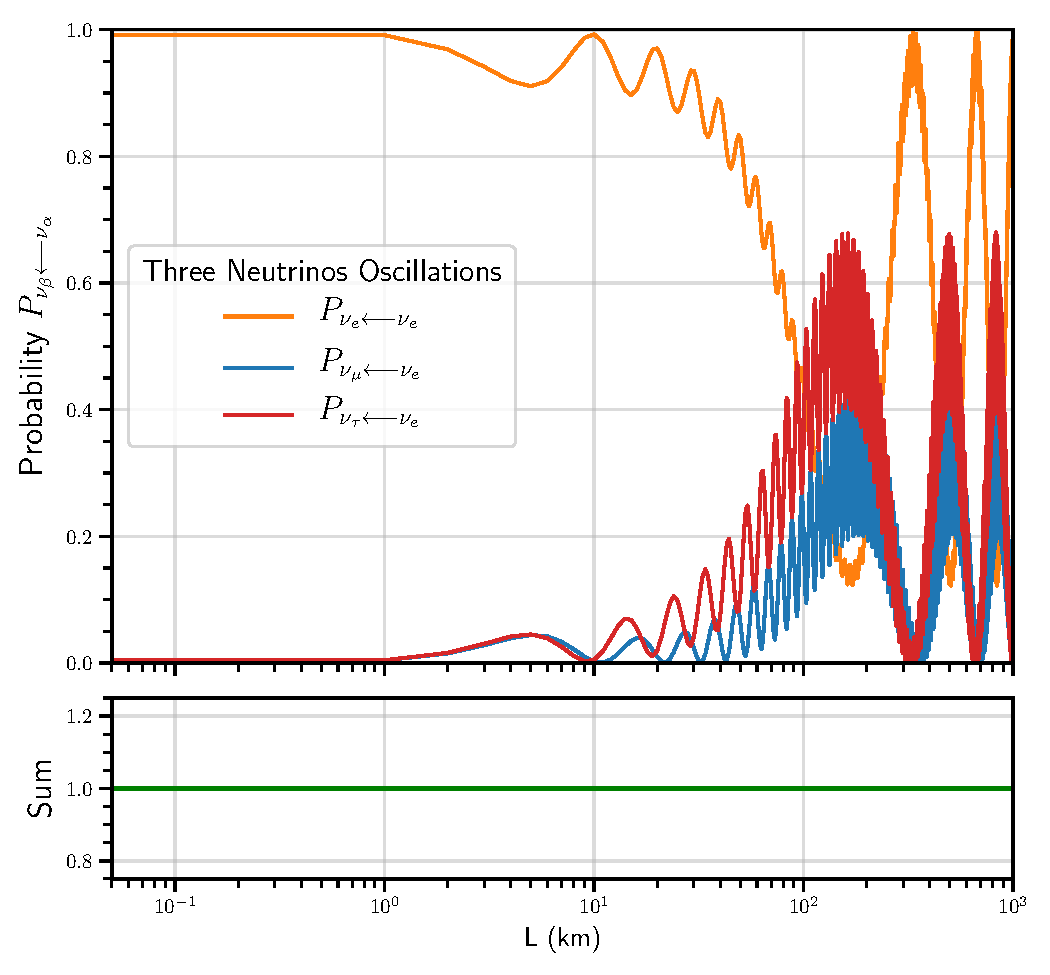
\includegraphics[width=\linewidth]{Osc3VacuumBaseline.pdf}
\caption{Varying baseline with fixed energy $E=10^{-2} \mathrm{GeV}$.} 
\label{higgs:sspt} 
\end{subfigure} 
\\
\begin{subfigure}{1.05\linewidth}
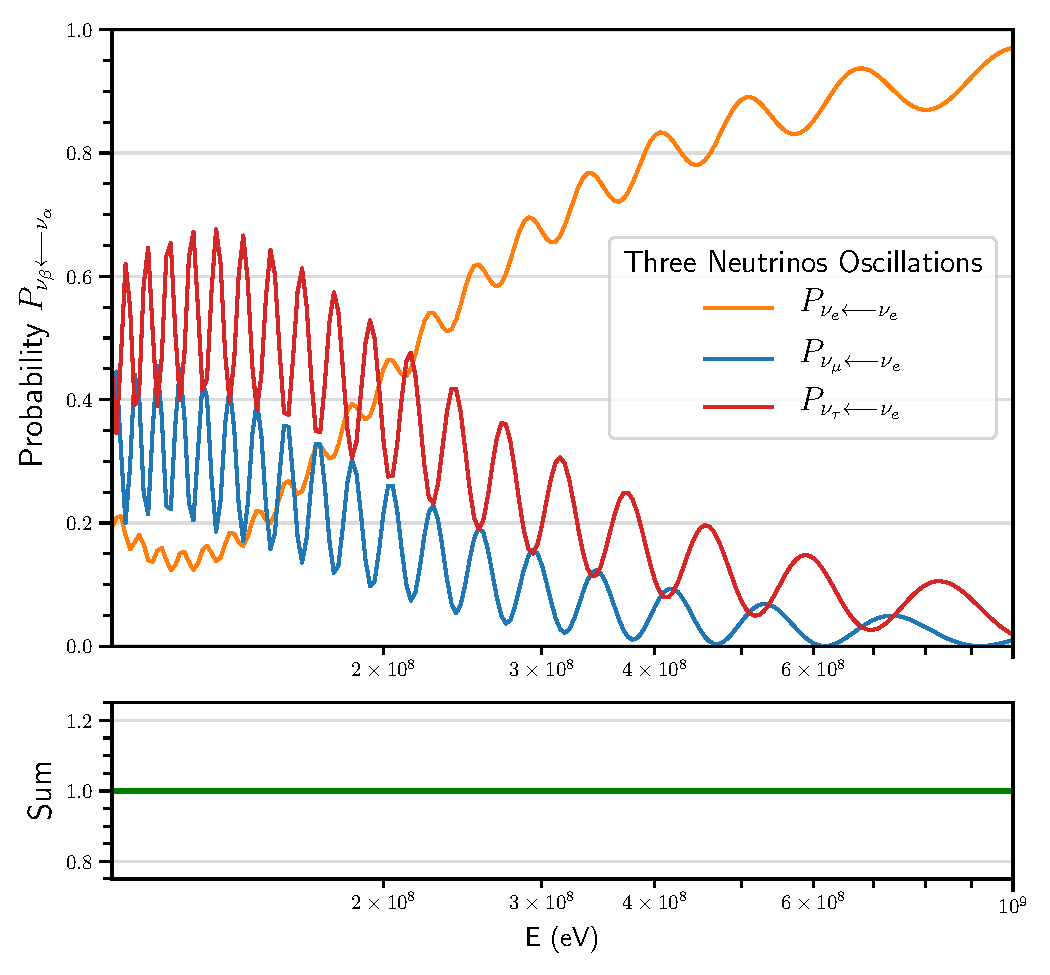
\includegraphics[width=\linewidth]{Osc3VacuumEnergy.pdf}
\caption{Varying energy with fixed baseline $L=2 \cdot 10^3 \mathrm{km}$.} 
\label{fig:vacuum} 
\end{subfigure}
\caption{Three-neutrino oscillation probabilities in vacuum with varying (a) baseline
and (b) varying energy. The top panels show the actual probabilities while the bottom
panels shown the sum of the probabilities which exactly sum to one.}
\end{figure}

In this project, we follow closely the method described in \myref{Bustamante:2019ggq} first 
introduced by Ohlsson and Snellman in Ref.~\cite{Ohlsson:1999xb, Ohlsson:1999um, Ohlsson:2001et}. 
It consists on expanding the Hamiltonian operator that enters in the expression of the evolution 
operator in terms of $SU(2)$ and $SU(3)$ matrices. The steps for such a calculation can be 
broken down into the following steps:
\begin{itemize}
\item[-] First, the Hamiltonian is expanded in terms of the Pauli matrices in the case of
two-neutrino oscillation, and in terms of the Gell-Mann matrices in the case of 
three-neutrino flavors.
\item[-] Compute the coefficients of the expansions in terms of the components of the
Hamiltonian.
\item[-] The exponent $\exp (\mathrm{i} H t)$ is then expanded using the Cayley-Hamilton theorem
which states that any analytic function of an $n \times n$ matrix can be written as a 
polynomial of degree $(n-1)$ in that matrix.
\item[-] Compute the evolution operator in terms of the coefficients in the Hamiltonian
series and derive the corresponding probability.
\end{itemize}
In this report, we only illustrate the case for two-neutrino oscillations. For the 
three-neutrino case, refer to \myref{Bustamante:2019ggq}. Let us denote the two-neutrino Hamiltonian
by $\mathrm{H}_2$. Its expansion in terms of the Pauli matrices $\sigma^i$ is given by
\begin{align}
\mathrm{H}_2 = h_0 + h_i \sigma^i \quad \quad (i=1,2,3).
\end{align}
The coefficients $h_k$ are fully determined by the components of the Hamiltonian matrix
and can be easily computed using the explicit expression of the Pauli matrices.
\begin{align}
\begin{array}{ll}
h_{0} =& \frac{1}{2}\left(\left(\mathrm{H}_{2}\right)_{11}+\left(\mathrm{H}_{2}\right)_{22}\right) \\
h_{1} =& \operatorname{Re}\left(\left(\mathrm{H}_{2}\right)_{12}\right) \\
h_{2} =& -\operatorname{Im}\left(\left(\mathrm{H}_{2}\right)_{12}\right) \\
h_{3} =& \frac{1}{2}\left(\left(\mathrm{H}_{2}\right)_{11}-\left(\mathrm{H}_{2}\right)_{22}\right)
\end{array}
\end{align}
The evolution operator $\mathrm{U}_2$ for the two-neutrino oscillations case can
therefore be written as
\begin{align}
\mathrm{U}_2 = \exp \left( - \mathrm{i} (h_0 + h_i \sigma^i) L \right).
\end{align}
The first term in the exponent does not affect the probability and therefore can be 
ignored. Hence, the evolution operator just becomes $\mathrm{S}_2 = \exp (- \mathrm{i}
h_i \sigma^i L)$. Using Euler's formula, the above expression yields
\begin{align}
\mathrm{S}_2 = \cos (\vert h \vert L) -  \frac{\mathrm{i}}
{\vert h \vert} \sin (\vert h \vert L) h_i \sigma^i ,
\end{align}
where $\vert h \vert = \sqrt{ \vert h_1 \vert^2 + \vert h_2 \vert^2 +
\vert h_3 \vert^2}$. We can now compute the survival probability 
\begin{align}
P (\nu_\alpha \longleftarrow \nu_\alpha) = \vert \nu_\alpha^\dagger \mathrm{S}_\alpha
\nu_\alpha \vert^2 .
\label{eq:prob_norm}
\end{align} 
Considering $\nu_\alpha = (1,0)^\mathrm{T}$, we can compute the terms that enter in the
expression of the probability in \Eq{eq:prob_norm}
\begin{align}
\nu_\alpha^\dagger \mathrm{S}_\alpha \nu_\alpha = \cos (\vert h \vert L) - \mathrm{i}
\frac{h_3}{\vert h \vert} \sin (\vert h \vert L).
\end{align}
Putting this expression back into \Eq{eq:prob_norm}, and with some algebras we can
derive the final expression of the survival probability of a neutrino of flavor $\alpha$,
\begin{align}
P (\nu_\alpha \longleftarrow \nu_\alpha) =  \cos^2 (\vert h \vert L) +
\frac{\vert h_3 \vert^2 }{\vert h \vert^2} \sin^2 (\vert h \vert L).
\end{align}
Therefore, the expression of the two-neutrino oscillation probabilities that a neutrino
of flavor $\alpha$ is detected with a flavor $\beta$ is given by the following simple
relation:
\begin{align}
P (\nu_\beta \longleftarrow \nu_\alpha) = 1 - P (\nu_\alpha \longleftarrow \nu_\alpha).
\end{align}

\begin{figure}
\captionsetup[subfigure]{aboveskip=-1.5pt,belowskip=-1.5pt} 
\begin{subfigure}{1.05\linewidth}
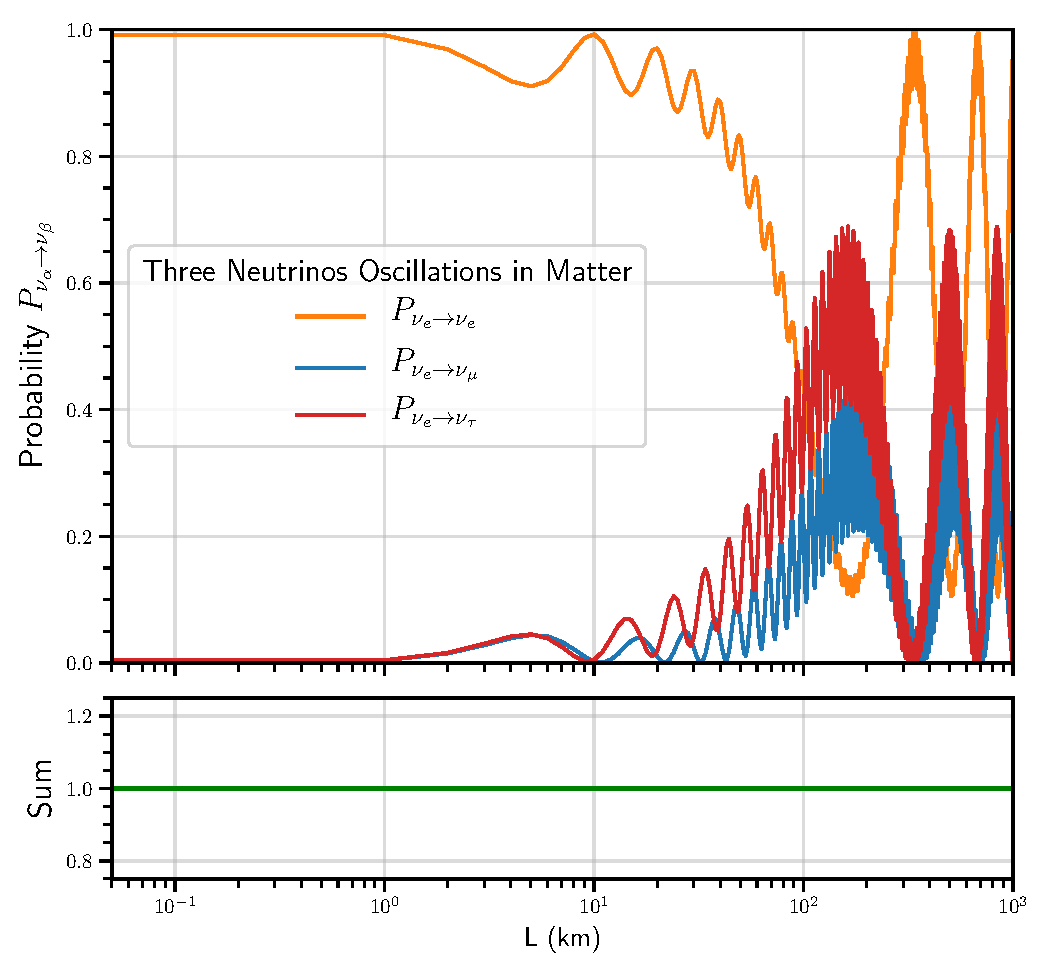
\includegraphics[width=\linewidth]{Osc3MatterBaseline.pdf}
\caption{Varying baseline with fixed energy $E=10^{-2} \mathrm{GeV}$.} 
\label{higgs:sspt} 
\end{subfigure} 
\\
\begin{subfigure}{1.05\linewidth}
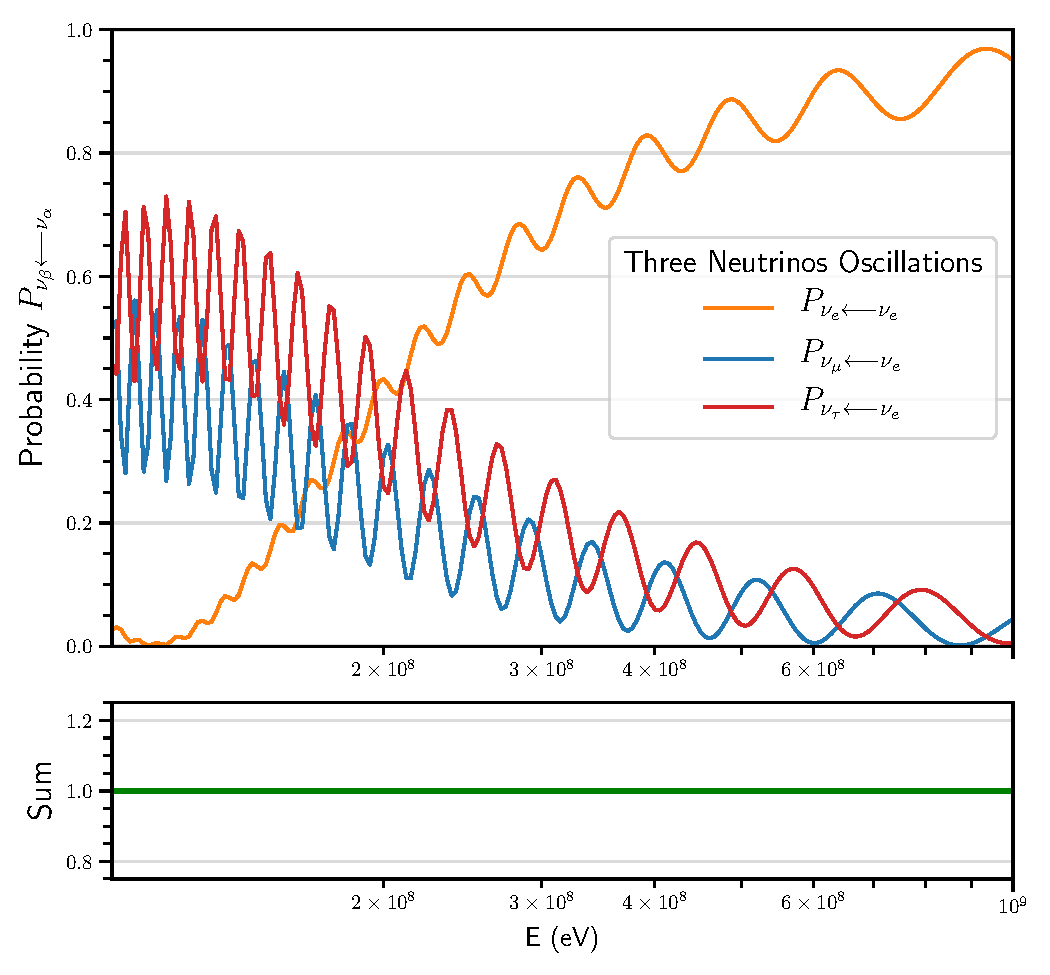
\includegraphics[width=\linewidth]{Osc3MatterEnergy.pdf}
\caption{Varying energy with fixed baseline $L=2 \cdot 10^3 \mathrm{km}$.} 
\label{fig:matter} 
\end{subfigure}
\caption{Three-neutrino oscillation probabilities in matter with varying (a) baseline
and (b) varying energy. The top panels show the actual probabilities while the bottom
panels shown the sum of the probabilities which exactly sum to one.}
\end{figure}

Let us now show that using this approach, we re-derive the two-neutrino oscillation
probability given by \Eq{eq:2OscProb}. For two-neutrino flavor oscillation, the vacuum
Hamiltonian operator is defined as
\begin{align}
\mathrm{H}_2^{vac} = \frac{1}{2 E} \mathrm{R}_{2, \theta} \mathrm{H}^{(m)}_2 
\mathrm{R}_{2, \theta}^\dagger ,
\end{align}
where $\mathrm{R}_{2, \theta}$ represents an Euler rotation with angle $\theta_{ij}$
and $\mathrm{H}^{(m)}_2$ is given by 
\begin{align}
\mathrm{H}^{(m)}_2 = \mathrm{diag} \left( \frac{\Delta_{ij}^2}{2}, - \frac{\Delta_{ij}^2}{2} \right). 
\end{align}
Using the coefficients $h_i$ to compute $\vert h \vert$, putting the explicit expression 
of the coefficients into \Eq{eq:prob_norm}, and doing some simplification, we arrive at 
the following expression
\begin{align}
P (\nu_\beta \longleftarrow \nu_\alpha) = \sin^2 (2 \theta_{ij}) \sin^2 \left(
\frac{\Delta_{ij}^2 L}{4 E} \right) ,
\end{align} 
which is exactly the same as in \Eq{eq:prob_norm}. The difference being that this approach
can be easily implemented numerically to compute oscillations in matter. Going into full
details of using this method to compute the three-oscillation probabilities and to study
neutrino oscillations in matter (including non standard oscillations) is beyond the scope of 
this project and will be left aside. For complete details and computations, refer to 
\myref{Bustamante:2019ggq}. The next section, however, will present results beyond the 
two-neutrino oscillations both in vacuum and in matter.


\subsection{Phenomenological results}
\label{subsec:results}

This section is dedicated to the phenomenological study of the three-neutrino oscillations
both in vacuum and in presence of matter with constant density. To compute the oscillation
probabilities, the only input parameters that we vary are the energy $E$ and the distance
traveled by the neutrino $L$. The other parameters such as the masses and the mixing angles
that enter in the expression of the PMNS mixing matrix are extracted from the NuFit code 
that fix the parameters to experimental data in order to find the best-fit values. These
parameters are summarized in Table \ref{tab:params}.
\begin{table}[!ht]
\centering
\begin{tabular}[t]{|c|c|}
\hline
\textbf{Parameters} 		& \textbf{Numerical Values} \\
\hline
$\delta_{CP}$			& $217^{\circ}$  \\
\hline
$\sin^2 \theta_{12}$		& $0.310$ \\
\hline
$\sin^2 \theta_{23}$		& $0.582$ \\
\hline
$\sin^2 \theta_{13}$		& $0.022$ \\
\hline
$\Delta_{21}$			& $7.391 \cdot 10^{-5}$ \\
\hline
$\Delta_{31}$			& $2.525 \cdot 10^{-3}$ \\
\hline
\end{tabular}
\caption{Numerical values of the mass differences $\Delta_{ij}$ and mixing angles
$\theta_{ij}$ extracted from a global fit to oscillation data \cite{Esteban:2018azc}.}
\label{tab:params}
\end{table}

The plots shown in this project were produced using python codes \cite{} which in turn rely
on an external python library called \texttt{NuOscProbExact} the numerical method 
presented in \myref{Bustamante:2019ggq}.

In \Fig{fig:vacuum}, we plot the three-neutrino oscillation probabilities as a function of
the baseline $L$ and energy $E$. In particular, we plot the probability that a neutrino
with an initial flavor $\nu_e$ oscillates between flavors $\nu_\beta$ (with $\beta = e,
\mu, \tau$). We can clearly see in the bottom panels that the sum of all probabilities
exactly gives one. For small values of $L$, we see that the probability that the 
electron-neutrino does not oscillate is high. As the neutrino traverses more distances,
this probability fluctuates, and in some regions smaller than the probability of the
neutrino to have a flavor $\nu_\mu$ or $\nu_\tau$. In the case of probabilities as a
function of energy with fixed baseline, we see that instead as the energy increases, the
probability that the neutrino keeps the same flavor is higher.
\begin{figure}
\captionsetup[subfigure]{aboveskip=-1.5pt,belowskip=-1.5pt} 
\begin{subfigure}{1.05\linewidth}
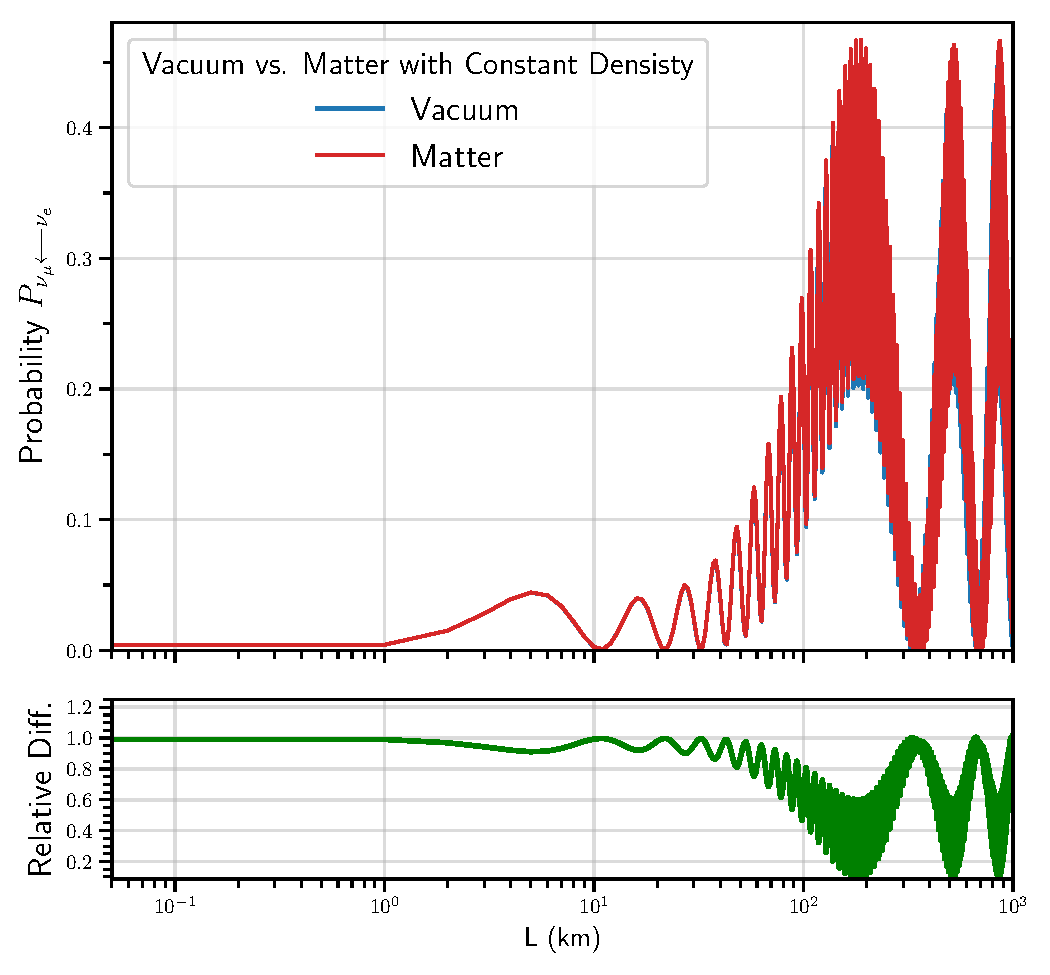
\includegraphics[width=\linewidth]{DistVacMatt.pdf}
\caption{Varying baseline with fixed energy $E=10^{-2} \mathrm{GeV}$.} 
\label{higgs:sspt} 
\end{subfigure} 
\\
\begin{subfigure}{1.05\linewidth}
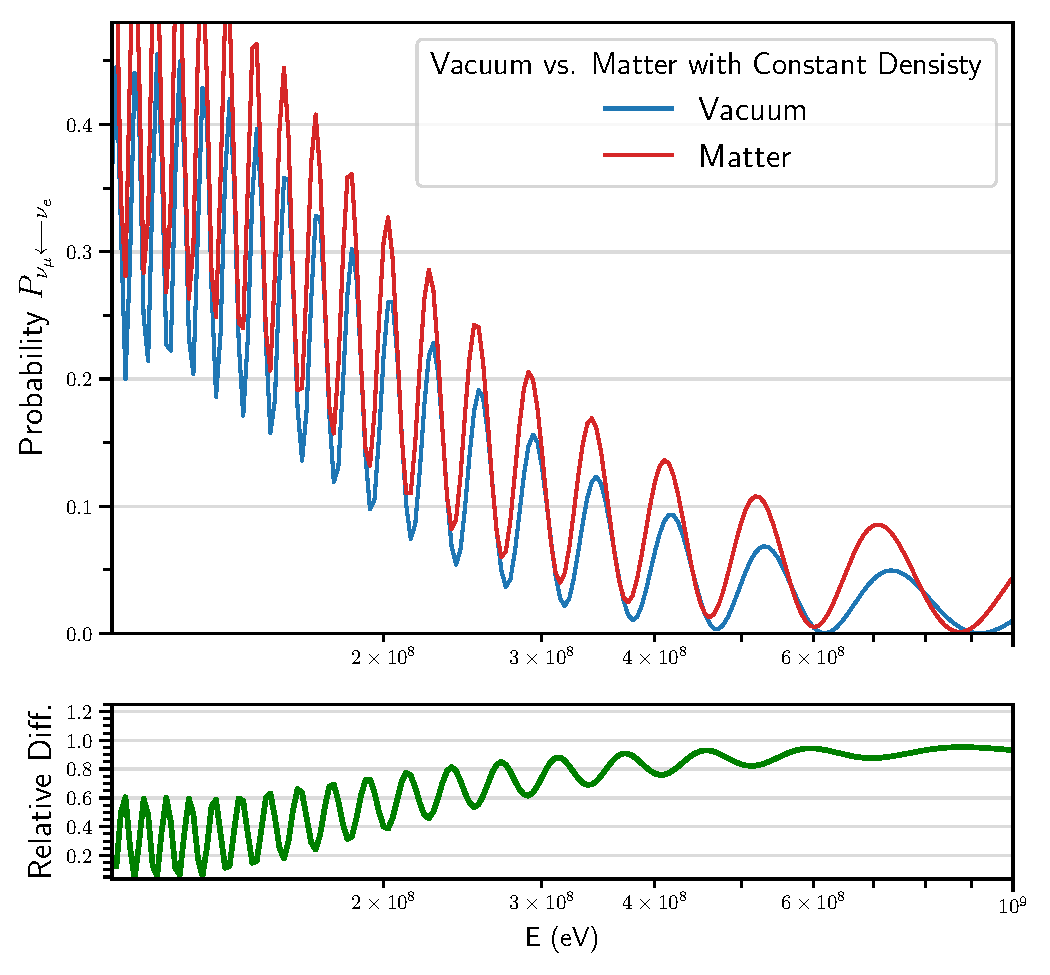
\includegraphics[width=\linewidth]{EngVacMatt.pdf}
\caption{Varying energy with fixed baseline $L=2 \cdot 10^3 \mathrm{km}$.} 
\label{fig:comparison} 
\end{subfigure}
\caption{Three-neutrino oscillation probabilities in matter with varying (a) baseline
and (b) varying energy. The top panels show the probability $\left( P_{vac} - P_{mat} 
\right) / P_{mat}$ both in vacuum and in presence of matter. The bottom panels plot
the relative differences.}
\end{figure}
In \Fig{fig:matter}, we show the three-neutrino oscillation probabilities for a neutrino
that propagates in a matter with constant density $\rho = 3 g/cm$. As we can see, the 
general behavior of the curves look similar to the propagation in vacuum. In order to
see the differences, we show in \Fig{fig:comparison} comparisons between propagation in
vacuum and in a matter for $P \left( \nu_\mu \longleftarrow \nu_e \right)$. The bottom
panels show the relative difference $\left( P_{vac} - P_{mat} \right) / P_{mat}$. We can
notice that for small distances (even at small energies), the matter has little effect
on the oscillation probability. It is worth mentioning that the propagation in a matter
with constant density is the simplest case and does not fully characterize realistic
scenarios. A more realistic scenario, for instance, is the study of a neutrino traversing
layers of matter, each with constant, but different density as in Ref.~\cite{Chizhov:1999az, 
Chizhov:1999he, Merfeld:2014cha}. Another well studied phenomena is neutrino oscillation 
with non-standard interactions. This takes into account the fact that the medium in which 
the neutrino is propagating in can affect its dynamics Ref.~\cite{Jacobsson:2001zk, Ohlsson:2003ip,
Arguelles:2012nw, Roe:2017zdw, Kelly:2018kmb}.


\section{Conclusion \& perspectives}
\label{sec:conclusion}

The fact that neutrinos have masses, which is a direct consequence of the neutrino oscillation,
is a concrete evidence of a physics beyond the current standard model (SM). This project attempted
to give a brief overview and introduction into the field of neutrino oscillation by focusing
mainly on the computation of the oscillation probabilities.

\Sec{sec:experiment} described the experimental probes of the neutrino oscillation phenomena that
led to its discovery. In \Sec{sec:theory}, we presented a condensed review of the theoretical 
framework behind the physics of neutrino oscillations. In particular, we focused on the analytical
computation of the oscillation probability (and survival probability). Then, in \Sec{sec:pheno} we 
presented some phenomenological results concerning the neutrino oscillation probabilities both as
a function of the energy and the baseline. We specifically studied the case for the three-flavor
oscillation. This has been achieved with the means of a numerical approach that overcome the problems
of diagonalizing the Hamiltonian in the analytical approach.

Albeit the field of neutrino oscillation physics has achieved quite some progresses in the last couple of 
decades, there are still many open problems that await to be unveiled. As briefly alluded in the
previous sections, some of the relevant issues concern the determination of neutrino mass 
hierarchy and the precise determination of the mixing angle $\theta_{23}$. The issue of mass
hierarchy might be resolved by the study of atmospheric neutrino oscillations as they are sensitive
to the mass ordering through matter effects for neutrino traversing the earth's atmosphere.
There are, on the other hand, issues that require high-precision experiments of not so immediate in future, such as the precise measurement of the Dirac-phase $\delta_{CP}$ and the probes of the CP violation in the leptonic sector. One of the prominent future experiments is the T2HK (Hyper-Kamiokande) that will be the successor of T2K \cite{Bellini:2013wra}. It is thus clear that high precision detectors
and reactors will play a crucial role in addressing these issues.

%%%%%%%%%%%%%%%%%%%%%%%%%%%%%%%%%%%%%%%%%%%%%%%%%%%%%%%%%%%%%%%%%%%%%%%%%%%%%%%%%%%%%%%%%%%%%%%%%%%%
%\nocite{*}
\bibliographystyle{unsrtnat}
\bibliography{biblio}


\end{document}

